\documentclass{article}
\usepackage[utf8]{inputenc}
\usepackage[a4paper, margin=1in]{geometry}
\usepackage[font={small,it}]{caption}
\usepackage{graphicx}
\usepackage{xcolor}
\usepackage{pdfpages}
\usepackage{natbib}
\usepackage{graphicx}
\usepackage{float}
\usepackage{url}
\usepackage{nameref}
\graphicspath{{../}}
\bibliographystyle{agsm}
\hyphenation{Vonnegut}

\title{\textbf{Using Natural Language Processing to Analyse the Shape of Stories}}
\author{
Luca Davies \\ B.Sc. (Hons.) Computer Science}
\date{20th March 2020}

\begin{document}
\maketitle
\newpage
\section*{TO DO LIST}
    \begin{itemize} 
        \item Redo Cinderella hand analysis (didn't store each individual sentence...) + write up anything interesting
        \item Comedy vs Tragedies (time permitting)
        \item Paul's Recommendations
            \begin{itemize}
                \item Create / include design diagram for Sentiplot sec design/dev
                \item Consider what to do about the bad-format input corpora from Gutenberg (re: section \ref{subsec:EMvME} and different length/block size), nothing I can do...?
            \end{itemize}
    \end{itemize}

\section*{Declaration}
    I certify that the material contained in this dissertation is my own work and does not contain unreferenced or unacknowledged material. I also warrant that the above statement applies to the implementation of the project and all associated documentation. Regarding the electronically submitted work, I consent to this being stored electronically and copied for assessment purposes, including the School’s use of plagiarism detection systems in order to check the integrity of assessed work. \\
    I agree to my dissertation being placed in the public domain, with my name explicitly included as the author of the work. \\
    
    \noindent
    Name: Luca Davies\\
    Date: 20/03/2020
\newpage
\section*{Abstract}
    This report examines the application of Natural Language Processing and Sentiment Analysis to fictional texts in an attempt to summarise narrative arcs as a curve on axes of time against positive/negative sentiment. VADER is used to process text for sentiment analysis and further experimentation is carried out to analyse how suitable VADER may be for this task. Corpora was mainly sourced from Project Gutenberg. A tool was developed to carry out a range of experiments on sentiment analysis that employed VADER as its sentiment analysis engine. Both quantitative and qualitative experimentation were carried out in the context of sentiment analysis around the following topics: the coarseness of sentiment analysis; the accuracy of VADER at sentence level via hand-tagging; sentiment analysis vs. analysis by human readers; early-modern English vs. modern English. It was found that Shakespearean texts proved difficult to process and so testing was also conduced using texts that had undergone spelling normalisation. It was discovered that a more powerful and versatile sentiment analysis engine would likely be needed to produce more readable curves and that a more flexible tool would prove useful for processing different text styles, such as scripts.
    \newline
    \newline
    Working documents such as source code, full experimentation results, early planning material and a full git history may be accessed at {\url{https://www.github.com/lucadavies/SCC300/}.
\newpage
\tableofcontents
\newpage
\section{Introduction}
    \subsection{Overview}
        Writer Kurt Vonnegut suggested at various points in his career that all stories may be categorised into a relatively small number of basic archetypes based upon the emotional ups and downs experienced within the narrative. He gave each of these novel names such as Man-In-Hole and Boy-Meets-Girl as a simple reference for each. \citep{vonnegutLecture}

        Literature is one of the defining features of the human race. No other creature on Earth can writes, let alone writes about itself. Humanity takes this a step further again, making up fictitious stories, some rooted in reality, some with no basis at all in which we dream and imagine worlds and situations that may never be possible to achieve. Through written word we express emotion. All emotions, happiness, sadness, anger and fear; love, hate, awe and grief – everything humans can feel, we write about. We create characters to express and receive these emotions, they act as vehicles to transfer their feelings to a reader. With all this freedom to write and create without bound, are we actually as free as we perceive?

        Vonnegut suggests that all stories are members of one of a very small number of categories of story that define roughly how the emotional progression of that story pans out. Do writers naturally and unknowingly write literature that falls into these types or is each story as unique as the next, taking its readers along its own path as they go?

        This concept and these questions drew me toward this project proposal. Not only is it a fascinating endeavour to map the emotions of a novel, but as an exploration of the freedom of writers to convey emotions and of how humans often generate categories and groups without even trying.

        With the high-level view clarified, it's important to note the types of tools within natural language processing that are relevant, namely that in this study, sentiment analysis takes the spotlight. Emotional analysis is a more in-depth field that shifts focus toward the psychological analysis \citep{sentimentVsEmotionAnalysis} and employs machine learning and artificial intelligence to further predict and understand the emotions presented in text.
        
        From a figures perspective, the basic process driving this project is as follows: a text is handed to a sentiment analysis tool which takes each sentence (or other identifiable section), processes it to produce a numeric value corresponding to that section's sentiment, then plots that value on an X-Y plot of sentiment values against progression through the text (e.g. by percentage along its course). This is basic premise of how the processing of corpora takes place. This is discussed in more detail in later sections.
    \subsection{Motivation}
        At it's core, this study is novel. It is interest driven - to attempt to show that stories can be categorised in a very simple and easy manner based upon the emotional arcs they lead readers across is an interesting new way to sort fiction. There may not be any explicit \textit{need} to categorise literature in this way, however it has the potential to lead to further studies that examine just how it is that humans create literature and any patterns we follow.

        As the project progressed, the goals shifted somewhat, leading to slightly differing aims, less focused on curve matching, and more on the use of natural language processing in literature as a whole. In some ways, the project was self-driven following initial results of attempting to identify curves. After it was proved difficult, the next steps naturally became to analyse quite why it was so difficult and to understand factors (such as the language and type of corpora used) that may be involved in the process.
    \subsection{Aims \& Objectives}
        The aims of this report are as such:
        \begin{itemize}
            \item Design and develop an application to process a range of corpora to produce a graphing of the emotional arc during its literary course (as produced using SA)
            \item Analyse a range of corpora for compliance with Kurt Vonnegut’s theories and story shapes
            \item Otherwise attempt to identify potential trends in the texts processed, such as obvious geometric differences between literature generally considered happy/sad
            \item Present graphs of texts to readers who are familiar with the text to assess if their perceptions of the text align with the SA graphs
            \item Assess VADER's ability to process text outside its design remit (e.g. early-modern English)
        \end{itemize}
    \subsection{Report Structure}
        The remainder of this report will discuss relevant background and context, the design and implementation of the Sentiplot tool, followed by a detailing of the experimentation carried out. The report will then be concluded by an analysis of the results acquired from this experimentation. \citep{reagan2016emotional}
\newpage
\section{Background}
\label{sec:background)}
    \subsection{Overview}
        This chapter will examine and summarise existing literature and studies in this area and topic. That is, natural language processing and sentiment analysis as a tool for extracting statistical data that describe emotions in (mainly) fictional works of literature.

        The processes involved for finding useful information included searching for online articles and pre-existing projects while searching libraries to use in the implementation, Google Scholar, Lancaster University Library OneSearch and Kurt Vonnegut’s own lectures on this topic.

        Existing projects will help to prove the developed application is performing up to standard (or not) and can be used as a side-by-side comparison of literature processed for this report and by these projects as well as to examine the processing of literature unavailable for the purposes of this report.
    \subsection{Natural Language Processing \& Sentiment Analysis}
        Natural Language Processing (NLP) is a very broad field concerned with, at a high level, the understanding of human language by computers. It fuses linguistics with computer science to not just parse but to \textit{understand} human language, to understand it in such a way that meaning can be deduced and emotion and sentiment can be extracted, even when not fully clear. More formally: ``Natural Language Processing (NLP) is an area of research and application that explores how computers can be used to understand and manipulate natural language text or speech to do useful things. NLP researchers aim to gather knowledge on how human beings understand and use language so that appropriate tools and techniques can be developed to make computer systems understand and manipulate natural languages to perform desired tasks.'' \citep{chowdhury2003natural}

        Via the beginnings of machine translation, NLP has existed as a research field for decades, even before the current name was coined. Breakthrough projects like ELIZA made progress in the field, but it wasn't until the 1980s that statistical methods began to be used. Prior to this, large sets of hand-written rules governed how NLP systems worked, which, although sometimes effective, limited the overall progress to the manual effort put into the models and rules. In modern NLP toolkits, models are still prevalent, but instead of them being assembled by hand, they are often formed using machine learning techniques based upon employing training data, test data and then real language data.

        Sentiment Analysis (SA) is a subfield of NLP that focuses on extracting and subsequently quantifying opinion and sentiment around a topic simply by analysing text. Accordingly, \cite{liu2012sentiment} describes Sentiment Analysis as: ``the field of study that analyses people’s opinions, sentiments, evaluations, appraisals, attitudes, and emotions towards entities \dots and their attributes.''
        
        By contrast to NLP, SA is a somewhat newer field, beginning to appear formally around the turn of the century. Likely it is that opinion mining has existed for a longer time in some form, `Sentiment Analysis' has only more recently started to appear in papers. Initial research concerned itself with extracting opinions from online product reviews. Overtime, with social media services like Twitter becoming prevalent, researchers have started to apply SA techniques to text taken directly from these services. As in the case of the Hedonometer Project (see \ref{subsec:hedonometer}, \cite{reagan2016emotional}), this data was then plotted against time to analyse general human opinion as a given point in time, linked in quite nicely to this project's mechanisms.
        With both NLP and SA garnering more and more interest in both the industrial and academic sectors, there are many all-in-one tools comprising both the NLP features required to perform SA but tools for conducting SA itself. Among these are Stanford CoreNLP (a full NLP suite, implemented via a pipeline model, \cite{stanfordNLP}), LIWC (a system with a focus on emotion for psychological analysis, \cite{tausczik2010psychological}), Natural Language Tool Kit (NLTK, a definitive tool set for nearly all NLP operations, \cite{loper2002nltk}), TextBlob (centred on text classification, built upon NLTK, \cite{textblob}), and multiple others. Many tools link between each other or are compiled from the bets performing sections of other tools. Some of these tools are standalone, and do not provide all NLP function in one package, instead trying to perform just a single function well - VADER (Valence Aware Dictionary and sEntiment Reasoner, \cite{hutto2014vader}) is a common tool for Sentiment Analysis, used in NLTK and elsewhere via the many language ports that have been written. As discussed in section \ref{subsec:nlpTools}, VADER was also the SA tool of choice for Sentiplot.

    \subsection{Kurt Vonnegut on ``The Shape of Stories''}
        Kurt Vonnegut described a number of potential story types as displayed below in figure something. He suggested that all stories fit into a very small number of categories, and moreover, that stories from different cultures around the world may generally trend toward different story types compared to elsewhere. In his lecture on the topic \citep{vonnegutLecture} Vonnegut draws out the curves of some well known novels and stories to demonstrate his meaning. Drawing distinct curves with very defined turning points and changes in direction that he claims match up with points in the given literature. This lecture was given a little later in his life, but the original concept stemmed from Vonnegut's rejected Master's thesis proposal presented to the University of Chicago. It was rejected by the University's Department of Anthropology on account of it seeming to simple and too much like fun. Consequently, it took a number of years before the topic was formally explored. Vonnegut's plans did however form the inspiration for this project as a whole, even if it has developed beyond his original ideas.
        \begin{figure}[htbp]
            \centering
            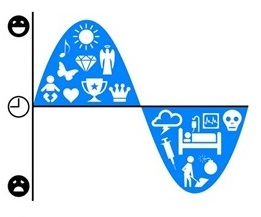
\includegraphics{Figures/Misc/sentimentGraph}
            \caption{Vonnegut suggest graphing sentiment in stories against narrative progression through the story.}
            \label{fig:sentiGraph}
        \end{figure}
        \begin{figure}[htbp]
            \centering
            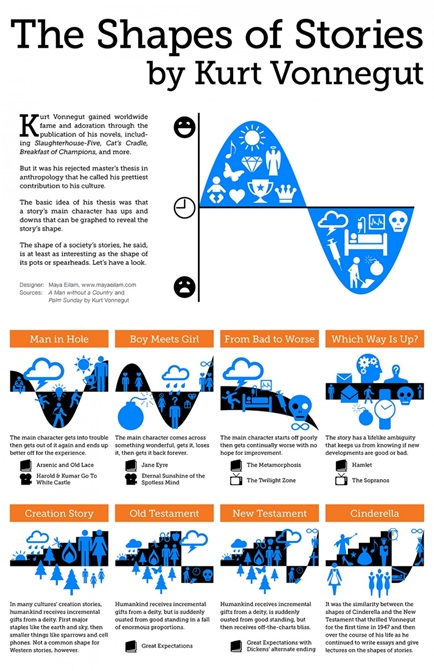
\includegraphics{Figures/Misc/VonnegutShapes}
            \caption{Vonnegut's Story Types, image from a digital article discussing Vonnegut's thesis \citep{vonnegutThesis}, information originally sourced from two of Vonnegut's own books \textup{A Man Without A Country} \citep{vonnegut_simon_2007} and \textup{Palm Sunday} \citep{vonnegut_1981}. Some of the Hedonometer Project's results show support for these curves.}
            \label{fig:storyTypes}
        \end{figure}
        
    \subsection{The Hedonometer Project}
    \label{subsec:hedonometer}
        The Hedonometer project was established to gauge happiness, the world over, starting with Twitter and other social media outlets. The project’s scope has since widened to process corpora direct from books, film scripts, news outlets and other foreign language literature. The overall premise is more vague than that of this study, aiming more generally to gauge happiness as a whole, but this naturally leads itself to measuring happiness against time, temporal or narrative. 
        Less complex techniques are used than most NLP and SA, instead using a bag-of-words approach, for example on 50 million random Tweets to assign a given day a score according to Twitter. The same type of method was applied to various classic novels, including all the \textit{Harry Potter} books. The results produced across all their various projects are very interesting and something this study hopes to replicate with more advanced techniques.
\newpage
\section{Sentiplot Tool}
\label{sec:sentiplot}
The experimentation required to undertake this study necessitated the need to develop a tool to process corpora and subsequently display it in a readable and analysable manner. The \textit{Sentiplot} tool filled this role: capable of parsing text from plain text files, Project Gutenberg formatted HTML and VARDed Shakespeare XML files (see section \ref{subsec:vard}). This section will detail the design and implementation of \textit{Sentiplot} during the course of the project. 
    \subsection{Languages \& Libraries}
    Within reason, any language could have been used to perform this study, however, ease of programmability and extendibility were also high up in the list of priorities. Familiarity with a given language and it's immediately available tools and APIs held significant sway during the selection process. Together with this, the appropriate NLP and SA toolkits had to be selected to provide a good balance between usability and performance which \textit{also} needed to be language compatible. This section briefly discusses the choice of programming language and NLP/SA tools used in the Sentiplot tool.
        \subsubsection{Top-level Language}
        \label{subsec:language}
        When selecting which language would be most appropriate to use for this project, my major considerations were my prior knowledge of potential languages and their ease of creation of a pleasant user interface. Availability of NLP tools in each language was also to be considered, but as the end implementation shows, this was not imperative due to cross-platform and cross-language capabilities of the chosen combination of languages and tools.

        A listing of considered languages follows:

        \begin{itemize}
            \item Java
            \begin{itemize}
                \item Strong language knowledge and familiarity
                \item JavaFX and Swing available for interfaces
                \item Native language of Stanford CoreNLP
            \end{itemize}
            \item Python
            \begin{itemize}
                \item Very limited language knowledge
                \item No knowledge of interface building
                \item Native language of industry standard NLTK
            \end{itemize}
            \item C\# (with .NET)
            \begin{itemize}
                \item Strongest language knowledge and familiarity
                \item Extreme ease in creating interfaces via Windows Form using Visual Studio
                \item Cross-platform variants of CoreNLP and VADER available via simple packages
            \end{itemize}
        \end{itemize}
        Taking all these points into consideration C\# was selected, due to its pros specific to myself and the availability of non-native libraries via APIs. This permitted me to use the full Microsoft Visual Studio suite for development, including the Windows Forms designer.
        \subsubsection{Natural Language Processing Tools}
        \label{subsec:nlpTools}
        Various tools across a wide array of languages are freely available to provide standard NLP functions and advanced processing capabilities.

        Initially a full CoreNLP pipeline was employed to process corpora but this proved to be extremely slow, loading around 2 gigabytes of models very slowly into memory before even processing anything. This is due to the various part-of-speech tagging and additional NLP tasks the pipeline had been setup to perform. These operation require usage of extensive models as reference for the application to run against. The pipeline was modified and optimised such that it only tokenised and sentence-split the input, and the actual sentiment analysis was performed by VADER.

        Both the CoreNLP and VADER libraries are non-native to C\# but have easy to use APIs for direct manipulation of their types and methods outside of their native environments. CoreNLP has an in-house developed API for C\# and VADER has a third-party API called \textit{VADERSharp}.
    \subsection{Design \& Development}
    \label{subsec:dnd}
        Sentiplot was developed over the course of two academic terms between early October 2019 and late January 2020. The first few weeks involved mainly research into what language was to be used and what NLP/SA tools or toolkits would provide the best mix of suitability-to-task and ease of use. The initial framework and basic features were developed using a waterfall type methodology before later, more experimental features were developed in a more ad-hoc manner using an agile development process after the main program with built. This approach was adopted based upon the time scales available: for the base application, a period of greater than a month allocated in which the bulk of programming needed to be carried out. It made sense to take this longer phase cautiously and slowly to ensure a quality code base to build features on top of in the next phase. In the feature development phase, additional smaller features were added to the Sentiplot application to facilitate the experiments (discussed in section \ref{experiments}). Each of these was initially allocated a development period of up to a ten days, much shorter than the previous phase, therefore it made sense to adopt a more agile, sprint-like methodology for each feature.
        
        The base application was projected to take 4-6 weeks to develop from scratch and the smaller experimental features added after to each take around a week. In reality, this first stage of development occupied the majority of the time from the start of November through till mid December. Then each of the experimental features pushed on from there, rolling into the next term, rather than all being finished before the Christmas holidays. Thankfully this did not cause major issues as there was an excess of time set aside for write up in the second term. Final bits of development including housekeeping and code styling wrapped up approaching week two of February 2020, still allowing time for this report write-up.

        As in discussed in section \ref{subsec:language}, C\# was the language used and Windows Forms was the user interface framework chosen. A full Visual Studio (Community) development suite was used to design, build and test the application which allowed for relatively swift and easy development due to the neat integration between the technologies. Had a different, less familiar language/framework been adopted, further schedule overruns may have occurred. StanfordCoreNLP was at one point the NLP tool of choice, however, difficulty and delay in marrying its Java libraries to C\# and setting up its processing pipeline are in large part what encouraged the eventual swap to VADER in early December.
        
        As the language and frameworks use lend themselves to it, the application is built with an object-oriented pattern in mind, however this doesn't come to light much as the application is somewhat self-contained - no other classes or applications need interface with it, Sentiplot only uses simple API calls to any external libraries.

        The overall internal structure of Sentiplot is not massively complicated. It is detailed in section \ref{subsec:implementation}.
    \subsection{Implementation}
    \label{subsec:implementation}
        \subsubsection{Structure}
            The application is written in C\# .NET interfacing with both Java and Python libraries via APIs as detailed in sections \ref{subsec:language} and \ref{subsec:dnd}. Windows Forms was chosen for the interface as a quick and easy to build platform, stable on Windows with seamless integration into C\# and the .NET framework.

            The application is composed of two forms, each with their designer code. The first allows the user to select a file to load text from and set processing granularity. The second presents the results of the analysis in multiple ways and provides facility to save these results as images of the output graphs.
        \subsubsection{Sentiplot Form (Main Form)}
            This is the main form for the application. It is loaded on start-up and contains all needed information or otherwise calls other classes to complete its task.

            Its key functions include:
            \begin{itemize}
                \item Initialising the CoreNLP pipeline to tokenise the input text
                \item Generating an OpenFileDialog object to allow the user to select a \textit{.txt} or \textit{.html} file
                \item Parsing the content of the input file to prepare it for processing using regular expressions and simple character-based splitting
            \end{itemize}
        \subsubsection{ResultsViewer}
            This form displays the results of VADER's processing of the input text. It displays a graph of the entire text from start to finish, a full list of all tokenised sentences and their associated sentiment scores (in tabular form) and individual graphs for each chapter in the text (HTML file only).

            \begin{itemize}
                \item Handling the output data and feeding it into the main chart and table
                \item Allow hiding/showing of each different type of sentiment score for the main graph
                \item Dynamically producing more tabs on the form to show each successive group of five chapters
            \end{itemize}
    \subsection{User Interface}
        The implemented interface did not need to be excessively complex or particularly appealing as it mainly served to function as a harness to conduct the study, with more importance placed on the code-behind and results.

        To provide quick results and ease of programming, I used the Windows Forms suite to produce a visually simple but functional interface. It has two screens: a screen to load the desired text to be processed and to set the granularity of the analysis, and a screen to present the processed results. The following sections provide an overview of these screens.
    \subsubsection{Text Selection \& Options}
    Figure \ref{fig:sentiplot} shows the main presented screen, after having loaded an HTML file (Hamlet in this case) which has been parsed to produce plain text, having stripped out all the unneeded HTML tags.
        \begin{figure}[htbp]
            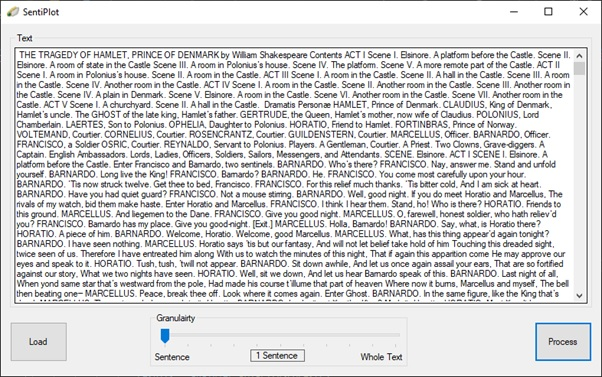
\includegraphics[width=1\textwidth]{Figures/Misc/sentiplot}
            \caption{Main Sentiplot window}
            \label{fig:sentiplot}
        \end{figure}
    \subsubsection{Results Display}
        Figure \ref{fig:resultsviewer} shows the results screen for \textit{Hamlet}, initially showing the graph of the entire text. The maximum and minimum points are labelled with the start of the related sentence. Hovering the mouse over these labels shows the entire sentence or sentences that produced that datapoint.

        For every sentence analysed VADER returns four sentiment scores: positive, neutral and negative (each holding a -1 to 1 score regarding match to that sentiment), and compound which acts as a single representation for the sentiment in the sentence parsed. Each of these scores have their own graph which may have their visibility toggled on and off with the check boxes in the bottom left. (Default is compound alone, as it proved the most indicative of sentiment, as advised by VADER documentation.) This graph can be saved to a JPG by clicking the save button.
        \begin{figure}[htbp]
            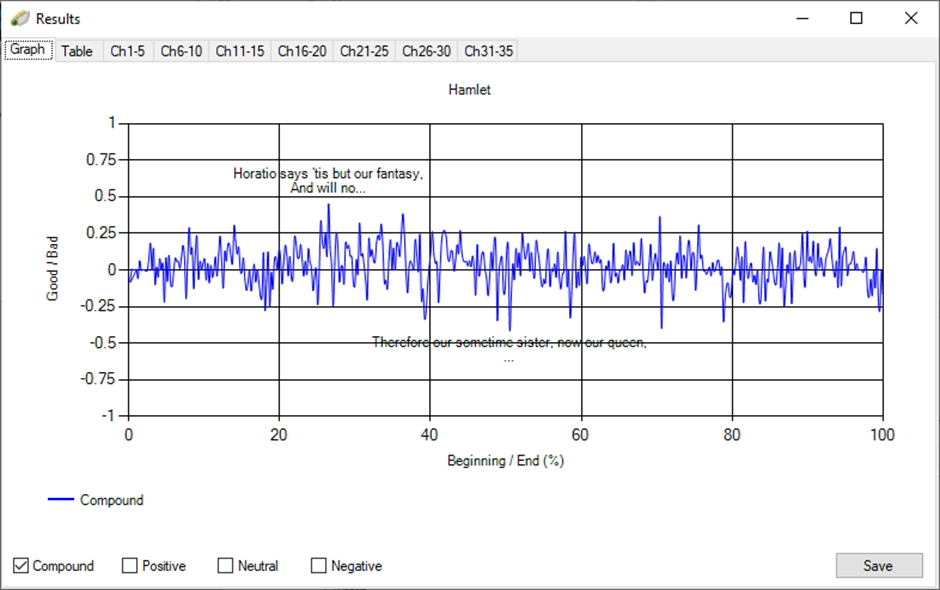
\includegraphics[width=1\textwidth]{Figures/Misc/resultsviewer}
            \caption{ResultsViewer window}
            \label{fig:resultsviewer}
        \end{figure}
        Figure \ref{fig:resultstable} shows the Table tab of the results screen. This simply lists each individual sentence token in the input with VADER’s output value for the four scores mentioned previously. The table’s default ordering in by sentence index, or the chronological order in the text, but the it may be order by any of the fields shown.
        \begin{figure}[H]
            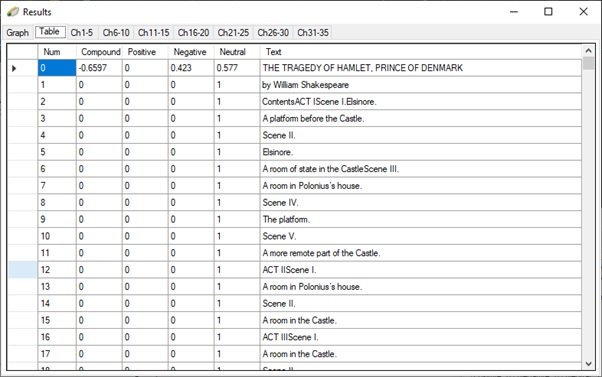
\includegraphics[width=1\textwidth]{Figures/Misc/resultstable}
            \caption{ResultsViewer window showing table}
            \label{fig:resultstable}
        \end{figure}
        Figure \ref{fig:resultschapters} shows one of the chapter tabs from the results screen. Each of graphs the compound sentiment score of up to 5 chapters from the processed text. Again, maxima and minima are labelled with their relevant sentence(s), expandable by hovering the mouse over the label.
        \begin{figure}[htbp]
            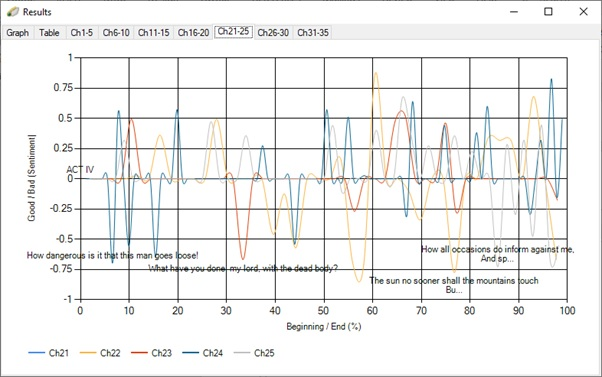
\includegraphics[width=1\textwidth]{Figures/Misc/resultschapters}
            \caption{ResultsViewer window showing chapter graphs}
            \label{fig:resultschapters}
        \end{figure}
    \subsection{Application Summary}
        The Sentiplot tool was used to acquire the majority of results detailed in section \ref{sec:experiments}. Written in C\#, utilising Stanford CoreNLP for basic NLP operations such as sentence splitting and tokenising, and VADER for the actual sentiment analysis. It provides functionality to process corpora raw or as provided by Project Gutenberg\footnote{For Project Gutenberg, see: \url{https://www.gutenberg.org/}} to an end of producing a graph or curve of the sentiment prevalent in the that text, with an option to control the granularity of that processing. The same processing is also carried out on a per-chapter basis where the input text allows.
\newpage
\section{Data}
    Having a tool to process a text is all well and good, but some input is of course required to produced any output. Throughout the process, considerations were being made with regard to what corpora was to be processed, graphed and examined. Much influence came from Kurt Vonnegut's lecture, mentioned in previous sections, in which he gave examples of well known stories for given curves. These included Cinderella, Metamorphosis and Hamlet, which were used for a majority of early testing of Sentiplot. The remainder came either from the image seem in figure \ref{fig:storyTypes} or were additional Shakespeare plays.

    Hamlet was the first Shakespeare processed, stemming directly from Vonnegut's lecture, but from there, processing more Shakespeare appeared to be a natural progression on account of it being so ubiquitously known. It also led nicely and easily into performing a qualitative study around perceptions of what curves of these plays could look like due to a number of personal connections with both English Literature, English Language and Theatre Students with a wealth of knowledge of the texts.
    
    \subsection{Selected Corpora}
    The following corpora have been subjects of this report. All were extracted directly from Project Gutenberg, with the exception of the VARDed texts which were provided by Jonathan Culpeper of the Linguistics and English Language Department, Lancaster University.
        \begin{itemize}
            \item Cinderella
            \item Metamorphosis
            \item Great Expectations
            \item Shakespeare
            \begin{itemize}
                \item A Midsummer Night's Dream
                \item Hamlet
                \item Macbeth
                \item Romeo and Juliet
                \item The Tempest
                \item Twelfth Night
            \end{itemize}
            \item Shakespeare (VARDed, see section \ref{subsec:vard})
            \begin{itemize}
                \item A Midsummer Night's Dream
                \item Hamlet
                \item Macbeth
                \item Romeo and Juliet
                \item The Tempest
                \item Twelfth Night
            \end{itemize}
        \end{itemize}
    \subsection{Variant Detector, VARD 2}
    \label{subsec:vard}
        The Shakespearean texts used present a problem unique to their age in the variety of different spellings for given words and the usage of highly unusual or archaic language. These variations can have a detrimental effect on the effectiveness of many NLP tools, particularly sentiment analysis, as unknown words may be ignored, or potentially worse, given a score opposite to what theory ought to be. In order to resolve this issue, these spellings must be normalised in a process dubbed ``VARDing'', named for the tool used to carry out the process: the Variant Detector tool, VARD (etymological origin from \textit{VAR}iant \textit{D}etector, \cite{baron2008vard2}) as produced during a study focussed on the tagging of historical corpora for use in NLP (see \cite{rayson2007tagging}). VARDed variants of the Shakespeare texts selected were acquired and parsed and it was these texts that were used in the early modern English vs modern English experimentation in section \ref{subsec:EMvME}.
    \subsection{Project Gutenberg Formatting}
    \label{subsec:gutenbergFormat}
            Chosen as the primary source of corpora, Project Gutenberg provides free, uncopyrighted literature for use in multiple formats. Early in development, Sentiplot had the capability to process plain text files only as this was deemed the simplest and easiest way to input text into the application. This was later found to be inadequate for the purposes of identifying and separately processing individual chapters.

            By chance, it was found that the HTML text provided by Project Gutenberg for both \textit{Macbeth} and \textit{Hamlet} (two of texts used to test the program during development) used HTML header tags to format Act and Scene numbers. It was also found that the preamble and postamble were enclosed in \mbox{\textless pre \textgreater \dots \textless /pre \textgreater} tags exclusively in this texts. An HTML file parser was then built in to Sentiplot to strip out unneeded information (pre/postamble, HTML tags, etc), decode it, and divide into chapter sections based upon these header tags. This worked for a number of texts, however, not all. It was taken for granted and assumed that Project Gutenberg used this as a standard format for all HTML file published - unfortunately this was not the case and sound of the graphs shown in this report are erroneous due to this.
            
            Some of the texts lack any chapters that are able to be analysed and most have multiple chapters that either contain a majority of preamble/postamble or, are a single line of text or whitespace.
\newpage
\section{Experimentation}
\label{sec:experiments}
The following section covers the various experimentation and analysis carried out on the selected corpora. A mixture of experiment types were carried out, some quantitative, looking at how produce the most readable output curve (see section \ref{subsec:blockSize} \nameref{subsec:blockSize}), others qualitative, surveying readers of the corpora what they thought the graphs should look like (see \ref{subsec:reader} \nameref{subsec:reader}), and some a mixture of both qualitative and quantitative methods, such as measuring the effectiveness of VADER by hand-scoring sentences that VADER has classified and comparing (see section \ref{subsec:handAnalysis}, \nameref{subsec:handAnalysis}). The different types of experiments were carried out in order to best represent and verify any and all findings.

    \subsection{Analysis Block Size}
    \label{subsec:blockSize}
        Sentiplot incorporates one primary setting for its analysis of texts: the granularity slider. This allows the user to select varying degrees of granularity for the produced graphs (as a percentage of the text being analysed). This allowed analysis of texts at a number detail levels to find which produced the most obvious curves to conform with Vonnegut's story curves. This may have introduced a small amount of positive-results bias, accepting those granularities that appear most curve-like for a given text instead of what may have actually reflected the curve of the text.

        The options provided and their effectiveness are shown in figure \ref{fig:granChart}.
        
        \begin{figure}[hbtp]
            \begin{center}
                \begin{tabular}{ |c|c|c| } 
                \hline
                \textbf{Too Fine} & \textbf{Acceptable} & \textbf{Too Coarse} \\ 
                \hline
                1 Sentence & 0.2\% & 5\% \\ 
                0.1\% & 0.5\% & 10\% \\
                & 1\% & 25\% \\
                & 2\% & 50\% \\
                &  & 100\% \\
                \hline
                \end{tabular}
            \end{center}
            \centering
            \caption{Various granularities are available for processing text, this table shows those that proved the most effective and those that did not.}
            \label{fig:granChart}
        \end{figure}
        This set of experiments varied the analysis block size for a given text and compared the output graphs for the entire text with a view to identifying a specific curve for the text. The comparison is qualitative, employing only human visual reference as opposed to any mathematical function. The purpose of this part of the study was as a forerunner to further analysis and experimentation to find the best setting or the best range of settings for either specific or generically for all texts to produce a coherent sentiment curve.
        \begin{figure}
            \includegraphics[width=1\textwidth]{Figures/Blocksize/Cinderella/cinderellaGran}
            \centering
            \caption{Each graph shows the result of decreasing the granularity of analysis and show how there appears to be a sweet spot. In this case, four of the highest options summed only a single sentence due to short length of the text. Only one of these has been included.}
            \label{fig:cinderellaGran}
        \end{figure}
        Figure \ref{fig:cinderellaGran} show the differing graphs that may be produced by changing the granularity.

        VADER is designed for parsing short lengths of text (less than 140 characters, as per a Tweet), so in order to produce more coarse graphs than single-sentence, VADER is still fed text on a per-sentence basis with the results summed up to \textit{N} sentences where \textit{N} is the corresponding number of sentences for a given granularity setting for a given text. The relevant data point is then plotted \textit{N} sentences beyond the previous (i.e. at the end of the analysed block).

        By default, every sentence of the text is plotted as its own point. This gives highly detailed graph but it very difficult to discern any sort of shape. Sentence to sentence, sentiment can vary wildly from the most negative in one to the most positive in the next (context and corpus dependent). Due to this, the resultant graph is highly spiked and difficult to garner information from.

        By contrast, using the more coarse options of 25\% and upward produce graphs that do show a clear line, the hope being the larger regions that have an average higher/lower sentiment score can then be picked out. However, at this level of coarseness, the data is compressed so much so that most of the detail is lost, smoothing the curve beyond useful limits for purposes of analysis

        Through trial-and-error experimentation, the ideal setting was found to lie between 0.2\% and 2\%, erring toward the 2\% for most texts. Although the choice to use percentages for the granularity setting was made to better cater to both long and short texts, those that are particularly long (>5000 sentences) and those that are particularly short (<200 sentences) may require different settings to best show the data and thus the curve. This is due to the fact that a longer novel does not necessarily have longer chapters and/or longer sections that could be identified as having a particular bias in sentiment.
        
        With all this being said, it's possible, that a different tool may have been better suited overall to this task than VADER is, due, at least in part, to it's native design choice to parse text the length of Tweets, not entire corpora. Sentiplot could be redesigned to pass VADER each block as a whole instead of summing the individual sentence values instead, although it is to be assumed that this would yield less accurate results as this is not how VADER was intended to be used.
    \subsection{Curve Identification}
    \label{subsec:curves}
        The original inspiration behind this project stemmed from Kurt Vonnegut's lecture on the ``The Shape of Stories'' and attempting to test his theory by plotting the sentiment results of various texts on a graph against time. This is what drove the initial development of Sentiplot and this study as a whole. However after initial results were produced by Sentiplot, one of two things became somewhat clear: either Vonnegut's theories were wrong, or VADER was not up to the task at hand. Which, remains to be seen and is likely best left to further research. Nevertheless, this meant that the aims of the project began to shift more toward NLP for processing literature in general (as opposed to its normal domain of opinion mining) and analysing those results. Consequently potential developments for curve identification were not developed to completion, namely, an algorithm to statistically compare the produced graphs with those predicted by Vonnegut, was never written. Despite this, mathematical plots were extracted from the six distinct curves mentioned in figure \ref{fig:storyTypes} (excluding `Which Way Is Up?' and `New Testament' for the fact of being a flat line and identical to `Cinderella', respectively) by using an online point plotting tool (see \cite{webPlotDigitizer}). The raw CSV data is provided in the additional documents to this report.

        Due to the above mentioned reasons, in-depth analysis into finding curves in corpora was scaled back compared to original plans. The following sections briefly explore the potential loose identifications of curves in a number of texts processed by the Sentiplot tool.
        \subsubsection{Whole Text Analysis}
            A small variety of both novels and scripts of varying lengths were processed to produce their curves. As mentioned above, there was not an immediately obvious correlations between many of the texts' graphs and those predicted by Vonnegut. 
            
            \textit{Great Expectations}, \textit{Metamorphosis} and \textit{Cinderella} were the three `novels' processed in decreasing order of length. \textit{Great Expectation} was the longest text processed with just shy of 10,000 sentence, however the only curve it could be sit to fit at face value is `Which Way Is Up?', or a flat line. There's variation, but only minor. Analysis of the curve from a larger perspective, one could argue it does \textit{almost} fit Vonnegut's predicted `New Testament' curve, albeit with an extremely reduced y-axis scale, and loss of all complex features of the graph. Kafka's \textit{Metamorphosis} shows a similar situation: the prediction is `From Bad To Worse', an ever decreasing parabola of sorts, however Sentiplot's output is at closest match, neutral, but at worst seems to have a few peaks and troughs of particularly negative \textit{and} positive sentiment. \textit{Cinderella} is the one graph that actually does bear somewhat of a resemblance to Vonnegut's prediction, being not too far removed from the rises and falls of his `Cinderella' curve, if slightly less extreme. See figure \ref{fig:cinderellaComp} for the produced graph overlaid with a representation of Vonnegut's curve transformed to fit the axes. The lack of the harsh drop at ~70\% may also be explained by the fact that block size averaging smooths out harsh changes such as this.
            \begin{figure}[hbtp]
                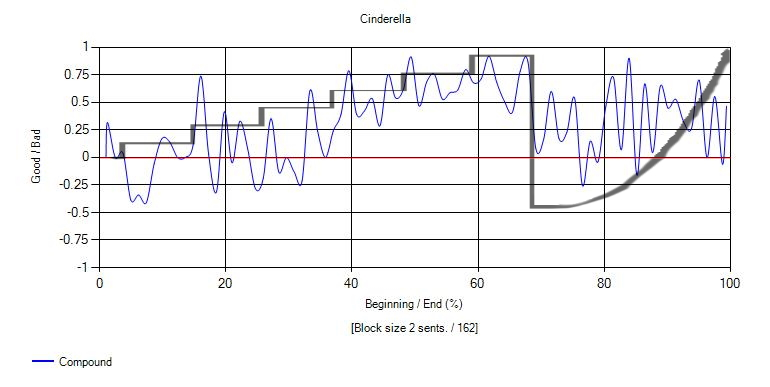
\includegraphics[width=1\textwidth]{Figures/Curve/CinderellaComp}
                \centering
                \caption{The curve produced for \textit{Cinderella} matches somewhat closely with Vonnegut's prediction.} 
                \label{fig:cinderellaComp}
            \end{figure}
            A number of Shakespeare plays were also processed in an initial attempt to match one of Vonnegut's suggestions in his lecture via the `curve' (supposedly a flat line) produced for \textit{Hamlet}. Although there were some minor exceptions, the majority of these texts produced highly restricted and unvarying graphs. The reasons for this are discussed in more detail in section \ref{subsec:reader}. Needless to say, this makes it very difficult to even begin to classify any of the curves according to any of Vonnegut’s types. Although unsuccessful at face-value, this prompted further experimentation in the form of section \ref{subsec:EMvME} in which modernised variants of the six plays are processed instead of the originals.
            \begin{figure}
                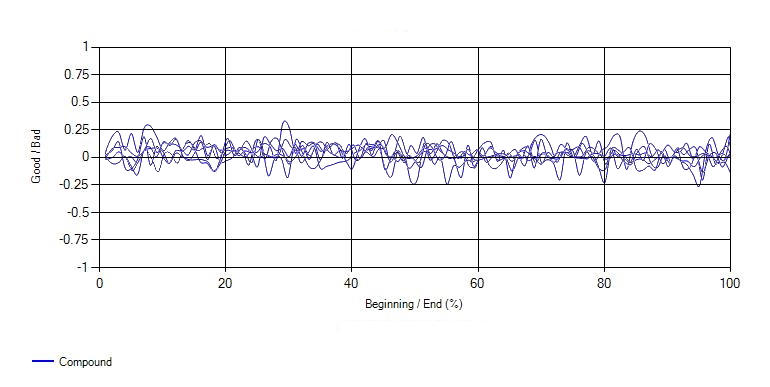
\includegraphics[width=1\textwidth]{Figures/Curve/ShakespeareOverlaid}
                \centering
                \caption{The graphs of six plays overlaid on top of one another. Rarely do any of the graphs exceed +/-0.25.} 
                \label{fig:ShakespeareOverlaid}
            \end{figure}
        \subsubsection{Chapter Analysis}
            This functionality was implemented in Sentiplot to further examine not only if stories had curves at all, but to see if any such curves could be discerned within smaller narrative sections of a larger text. The method is not greatly complex, dividing a text into chapters and simply graphing and plotting each chapter individually to ease analysis.

            Each chapter is plotted using the same granularity as the main text, this being a percentage of the input text length. Here, this percentage is applied to the length of the chapter itself. Depending on average chapter length this can mean that specific a granularity may have to be chosen to examine chapters. Being much shorter than the full text, the 1\% often used for a whole text can lead to single-sentence processing for many chapters and thus yield erratic graphs.
            \begin{figure}
                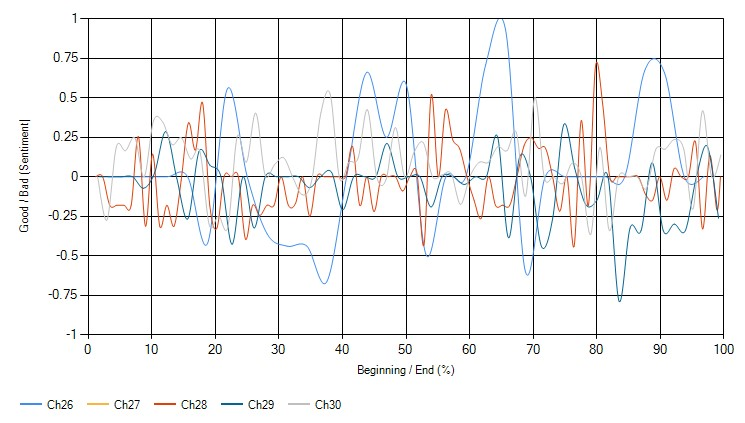
\includegraphics[width=1\textwidth]{Figures/Chap/Macbeth}
                \centering
                \caption{``Chapters'' 26 to 30 of \textit{Macbeth} showing five overlaid curves. Chapter 26 (light blue) shows potential shape albeit somewhat extreme.} 
                \label{fig:macbethChap}
            \end{figure}
            Figure \ref{fig:macbethChap} shows one of the chapter tabs from processing \textit{Macbeth} with a higher percentage granularity than would normally be used, for the sake of giving useful results in the chapters screen. It can be seen here that there is a potential for curves to be found here, though given the majority negative results elsewhere, it's highly likely any matches would be either coincidence or subject to positive-result bias.
    \subsection{Hand Analysis Vs. VADER}
    \label{subsec:handAnalysis}
        This test was performed by selecting a 100 random sentences from two texts (Macbeth and Cinderella), analysing them each individually by hand and estimating a combined positive/negative sentiment score in the same range as that produced by VADER. I attempted to avoid trying to emulate the way VADER would process the text, instead scoring each sentence as I would as a reader of the text: "Would I feel positively and negatively after reading this sentence?" or, similar - a human approach.
        
        The motivation behind this was to understand if VADER's output results were trustful, totally incorrect, or somewhere in the middle. It's easy to blindly follow what a program says but NLP and Sentiment Analysis is still very much a field that cannot yet directly emulate the processes of the human brain.
    
        \begin{figure}[hbtp]
            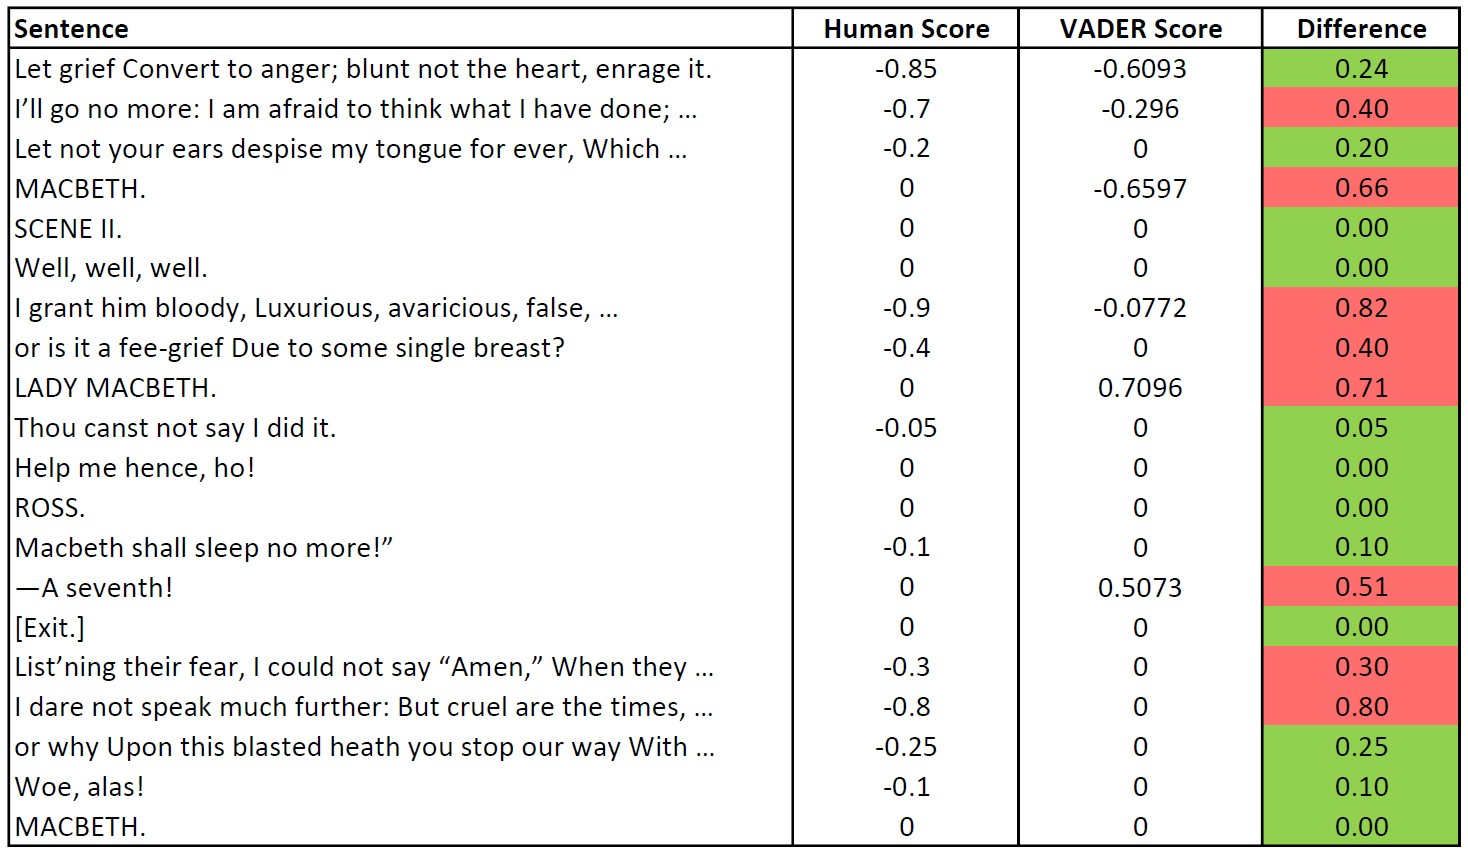
\includegraphics[width=1\textwidth]{Figures/HandAnalysis/Macbeth}
            \centering
            \caption{An excerpt from the table of human-analysed sentiment scores along side VADER's scores with the difference (highlighted green for a match, red otherwise) shown. The original sentences from \textit{Macbeth} are shown for reference.}
            \label{fig:handMacbeth}
        \end{figure}
        
        The results obtained, although they are based on one person's own judgement (and hence are not necessarily reliable), were disappointing to say the least. To determine similarity, a threshold difference of +/-0.25 was chosen to mark the boundary between results that correlated with each other, and results did not. From this, of the 100 sentences taken from Cinderella, only 27\% matched. In the case of Macbeth, 50\% matched, but it is possible to theorise that majority of the increase is likely due to the fact of \textit{Macbeth} being a script - namely, there were many sentences that were just a name, or just a stage direction alone and thus was very easy to be rated neutral (or, zero) by both a human and VADER. However, in the 100 sentences, 29 names, stage directions or similar were present, of which 10 matched (mainly at or near zero), decreasing the effective percentage of matched sentences to somewhere in the range 21\%-40\%. There were some cases where a plain name resulted in an extreme score (see rows 4 and 9 in figure \ref{fig:handMacbeth}). Some of the scores assigned by VADER also seem to make little to no sense whatsoever, for example, row 7 in figure \ref{fig:handMacbeth}: the full sentence directly includes (without negation), the words ``bloody'', ``avaricious'', ``false'', ``deceitful'', ``malicious'', and ``sin'', and yet VADER scores the sentence all but neutral, while most human readers would likely rate this one of the most negative in the data set.

        Though not in the previous example, it is possible that some of these erroneous results may stem from the fact that the way VADER is being utilised in Sentiplot means that it has no context for any given sentence, they are all processed stand-alone and so VADER cannot build up any running themes or patterns to aid in analysis.

        To conclude, this experiment raised potential issue with the usage of VADER, suggesting an alteration in Sentiplot's implementation but also questioned the overall effectiveness of VADER as a sentiment analysis tool given some rather unusual results upon close inspection. The next section partially opens up this discussion to a wider audience, allowing comment on the final results produced by VADER and some comments on its processes.
    \subsection{Reader Analysis \& Reflection}
    \label{subsec:reader}
        This section covers the analysis of a range of Shakespeare plays by human readers (mostly identified to be Theatre and/or Literature students) and their personal comparison of the the Sentiplot output with their own expectations of what a graph of a given play should be. The goal here was to bring a human element to the reviewing of Sentiplot and VADER. A brief background of the study, its goals, and task was given to each person who answered any of the questions provided. Some asked further questions and subsequently commented on the techniques used for analysis and graph production.
        \subsubsection{Reader Analysis}
            Readers were first asked if they felt they knew each play well enough to attempt to plot a rough arc for each on a set of axes, with a focus on any major emotional events they could identify. Some participants opted to answer questions on only a subset of the plays, as they may not have read or otherwise cannot remember the other plays. In total, 22 result sets were gathered. This allows qualitative analysis to be carried out around how effectively VADER performed from a human perspective and to attempt to gather further comment from participants on the effectiveness of Sentiplot.

            Each participant was given a blank set of axes (with the same scale as was used for VADER's results). They were asked to draw what they thought a curve of each play would look like, based upon any and all major events they can recall. They were then asked to label and/or explain any notable peaks and troughs in their curves. A small selection of the curves drawn are shown in figure \ref{fig:readerVsVader}, paired with the corresponding output form VADER.
            \begin{figure}[htbp]
                \includegraphics[width=1\textwidth]{Figures/Survey/readerVsVader}
                \centering
                \caption{Readers (top of each pair) in general drew curves bearing little to no similarity to those produced by VADER (bottom in each pair)}
                \label{fig:readerVsVader}
            \end{figure}
            In general, all the curves drawn by participants were wildly different to the VADER output for the same texts. All VADER's curves stayed mostly in the range of +/-0.25 on the Sentiment axis, whereas most participants drew curves using nearly the full extent of the y-axis. It was to be expected that participants would use the full axis, but it was not expected before setting out on this experiment that VADER's graphs would be quite so restricted. This is not to say that VADER doesn't register any sentences as reaching the more extreme values: when examining the per-sentence scores in the table view, it does, but these values get flattened when they are grouped together. On closer inspection, taking \textit{Macbeth} as an example, approximately 30\% of the sentences were outside the +/-0.25 range, however  just over 60\% of those \textit{within} that range were zeros: registered by VADER as completely neutral sentences. When taking averages, these high volumes of zero-scored sentences reduced the impact on the output graph of higher scores greatly.

            Even with this failure, attempting to look at relative differences along the two curve sets (those drawn, and those produced by VADER) still doesn't yield much similarity. The only immediately obvious correlation is, again, in \textit{Macbeth} where both VADER and a participant show a sharp dip at around the halfway mark (labelled on the drawn curve as "murder"). This is nearly the only obvious match.
            
            Kurt Vonnegut suggested in his lecture that \textit{Hamlet} ought to have a somewhat flat curve. Sentiplot supports this at least visually, however, some of the drawn graphs show a very clear descent, logically coupling Hamlet's madness with negative sentiment. Sentiplot does in fact also show some extreme peaks and troughs, however these are momentary in the overall context of the script, and thus are averaged out and do not appear in the final output. Depending on the scope at which you examine, but Sentiplot has elements of agreement with both Vonnegut's flat prediction \textit{and} participant's more curved graphs.
			\subsubsection{Reader Reflection}
                Participants were later asked to comment on the similarity (or dissimilarity) between their own graphs and those from VADER. There was a general consensus that VADER's graphs lacked the ability to show various details and intricacies of the literature or were otherwise just plain wrong. 
                One participant noted the failure of the system pickup on tonal dissonances within a \textit{A Midsummer Nights Dream} - this is assumedly a reference to the multiple plot lines within the play and their sometimes conflicting emotional tones. If VADER had a greater capability to distinguish plot lines and characters within a text from one another, it's highly likely that each plot within a text would have its own curve.
                
                It was also said that the Sentiplot graphs failed to pick up on even the extremities of character emotions (namely in \textit{Romeo and Juliet}) and also in the overall tone of a play (Hamlet, showing as being relatively neutral when expected to be generally negative).

                Another participant mentioned that they felt undertones in the text were totally lost in the graphs (though this is perhaps to be expected) and that they failed to differentiation between specific known periods of happy/sad narrative segments. One specific example of this is seen at the end of \textit{Romeo and Juliet} - a decidedly negative section of literature, at least at surface level. Of the two responses for \textit{Romeo and Juliet} received, both finish the play below zero, with one plummeting the sentiment score down to maximum negative. By contrast, VADER's graph actually \textit{rises} at the end, the second highest point in the entire graph. This is a major error, of course, but after seeing the results, the text processed was examined closer and it was found that Sentiplot had failed to strip out the sizable Project Gutenberg pre- and postamble in the processed HTML file. It was the postamble (making up the final 5\% of the text) that gave rise to this upward spike where there was otherwise a negative trend that met readers expectations. Unfortunately it was found that this was not an isolated issue and is covered in more detail in section \ref{subsec:gutenbergFormat}.
                
                A few participants noted that some of VADER's graph appeared to have little to no correlation with the text at all, with some attributing this to a computer program's lack of the ability to experience or empathise with literary art. It was also suggested that a theatrical script is likely to be a less than ideal format for attempting to produce a curve in this way, with one participant pointing out that scripts do not contain significant amounts of description - they only contain dialogue, with a small (albeit, varying) amount of description present in the stage directions; novels on the other hand innately contain description as it is the primary information is conveyed to the reader.
    \subsection{Early Modern Vs. Modern English}
    \label{subsec:EMvME}
        In this experiment, VARDed (see \ref{subsec:vard}) variants of six Shakespearean plays were processed by Sentiplot. The VARDed texts are modern English variants of Shakespeare's texts, the goal here being to compare just how much of an impact the difference in language (early-modern English vs. modern English) has on the ability of VADER to analyse sentiment.

        VADER is not trained to work on the likes of formal literature. In fact, it is trained to work on highly modern and informal text, to such an extent that it can understand and analyse Internet slang and emoji. Due to this fact, this experiment was carried out to test if VADER was able perform equally or at all as well on a different form of English, that being the Early Modern English found in the Shakespeare plays processed for section \ref{subsec:reader}. The assumption is that VADER will perform better on modernised texts, as that is what its models have been trained to process.
        
        The original Project Gutenberg texts of the plays gave graphs that did not hold much variation - processing the modernised text overall gave similar graphs at first glance, similar but with exaggerated peaks and troughs with the overall form is still held. However, finer inspection will show that in fact, there's a number of new features visible in most plays that were not present in the original text. For example: in the latter 40\% of the original text of \textit{The Tempest}, the graph has less variation, staying practically in the range of zero to 0.1 - in direct opposition, the varded text has a number of sizable peaks and troughs, with a maximum magnitude score of approximately positive 0.3. Similarly, in \textit{A Midsummer Nights Dream}, just after the halfway mark, there appears to be a fairly distinctive negative period for a while, a feature that isn't shown at all on the original text (in fact, it appears to go become more \textit{positive}).\footnote{It should be noted in \ref{fig:emvsm} that there are discrepancies between block size and text length between the original and VARDed texts. Both sets were processed at 1\% granularity, however the VARDed texts lack characters names in the main body of the text, as opposed to the original where they are in line. Character names were manually removed from \textit{The Tempest} for a unique test to see if this had a significant impact on the output results. The original and the version without names produced very very similar graphs, therefore it may be assumed that the differences observed in this experiment are primarily a result of the spelling normalisation.}

        These new additions seen in most graphs demonstrate VADER's limited ability to process early modern English text, causing it produce values erring much more toward neutral zero-values than it should. This is understandable as the many words used in early modern English It is still reasonable to attribute the restricted nature of the these original graphs, at least partially, to the nature of the text, them being scripts, not novels, however it can still be seen that processing modern English is gives more meaningful results. This is evidenced in the huge variation (nearly full -1 to 1) of the graph of \textit{Cinderella} in figure \ref{fig:cinderellaGran} which is also written in modern English.
        \begin{figure}
            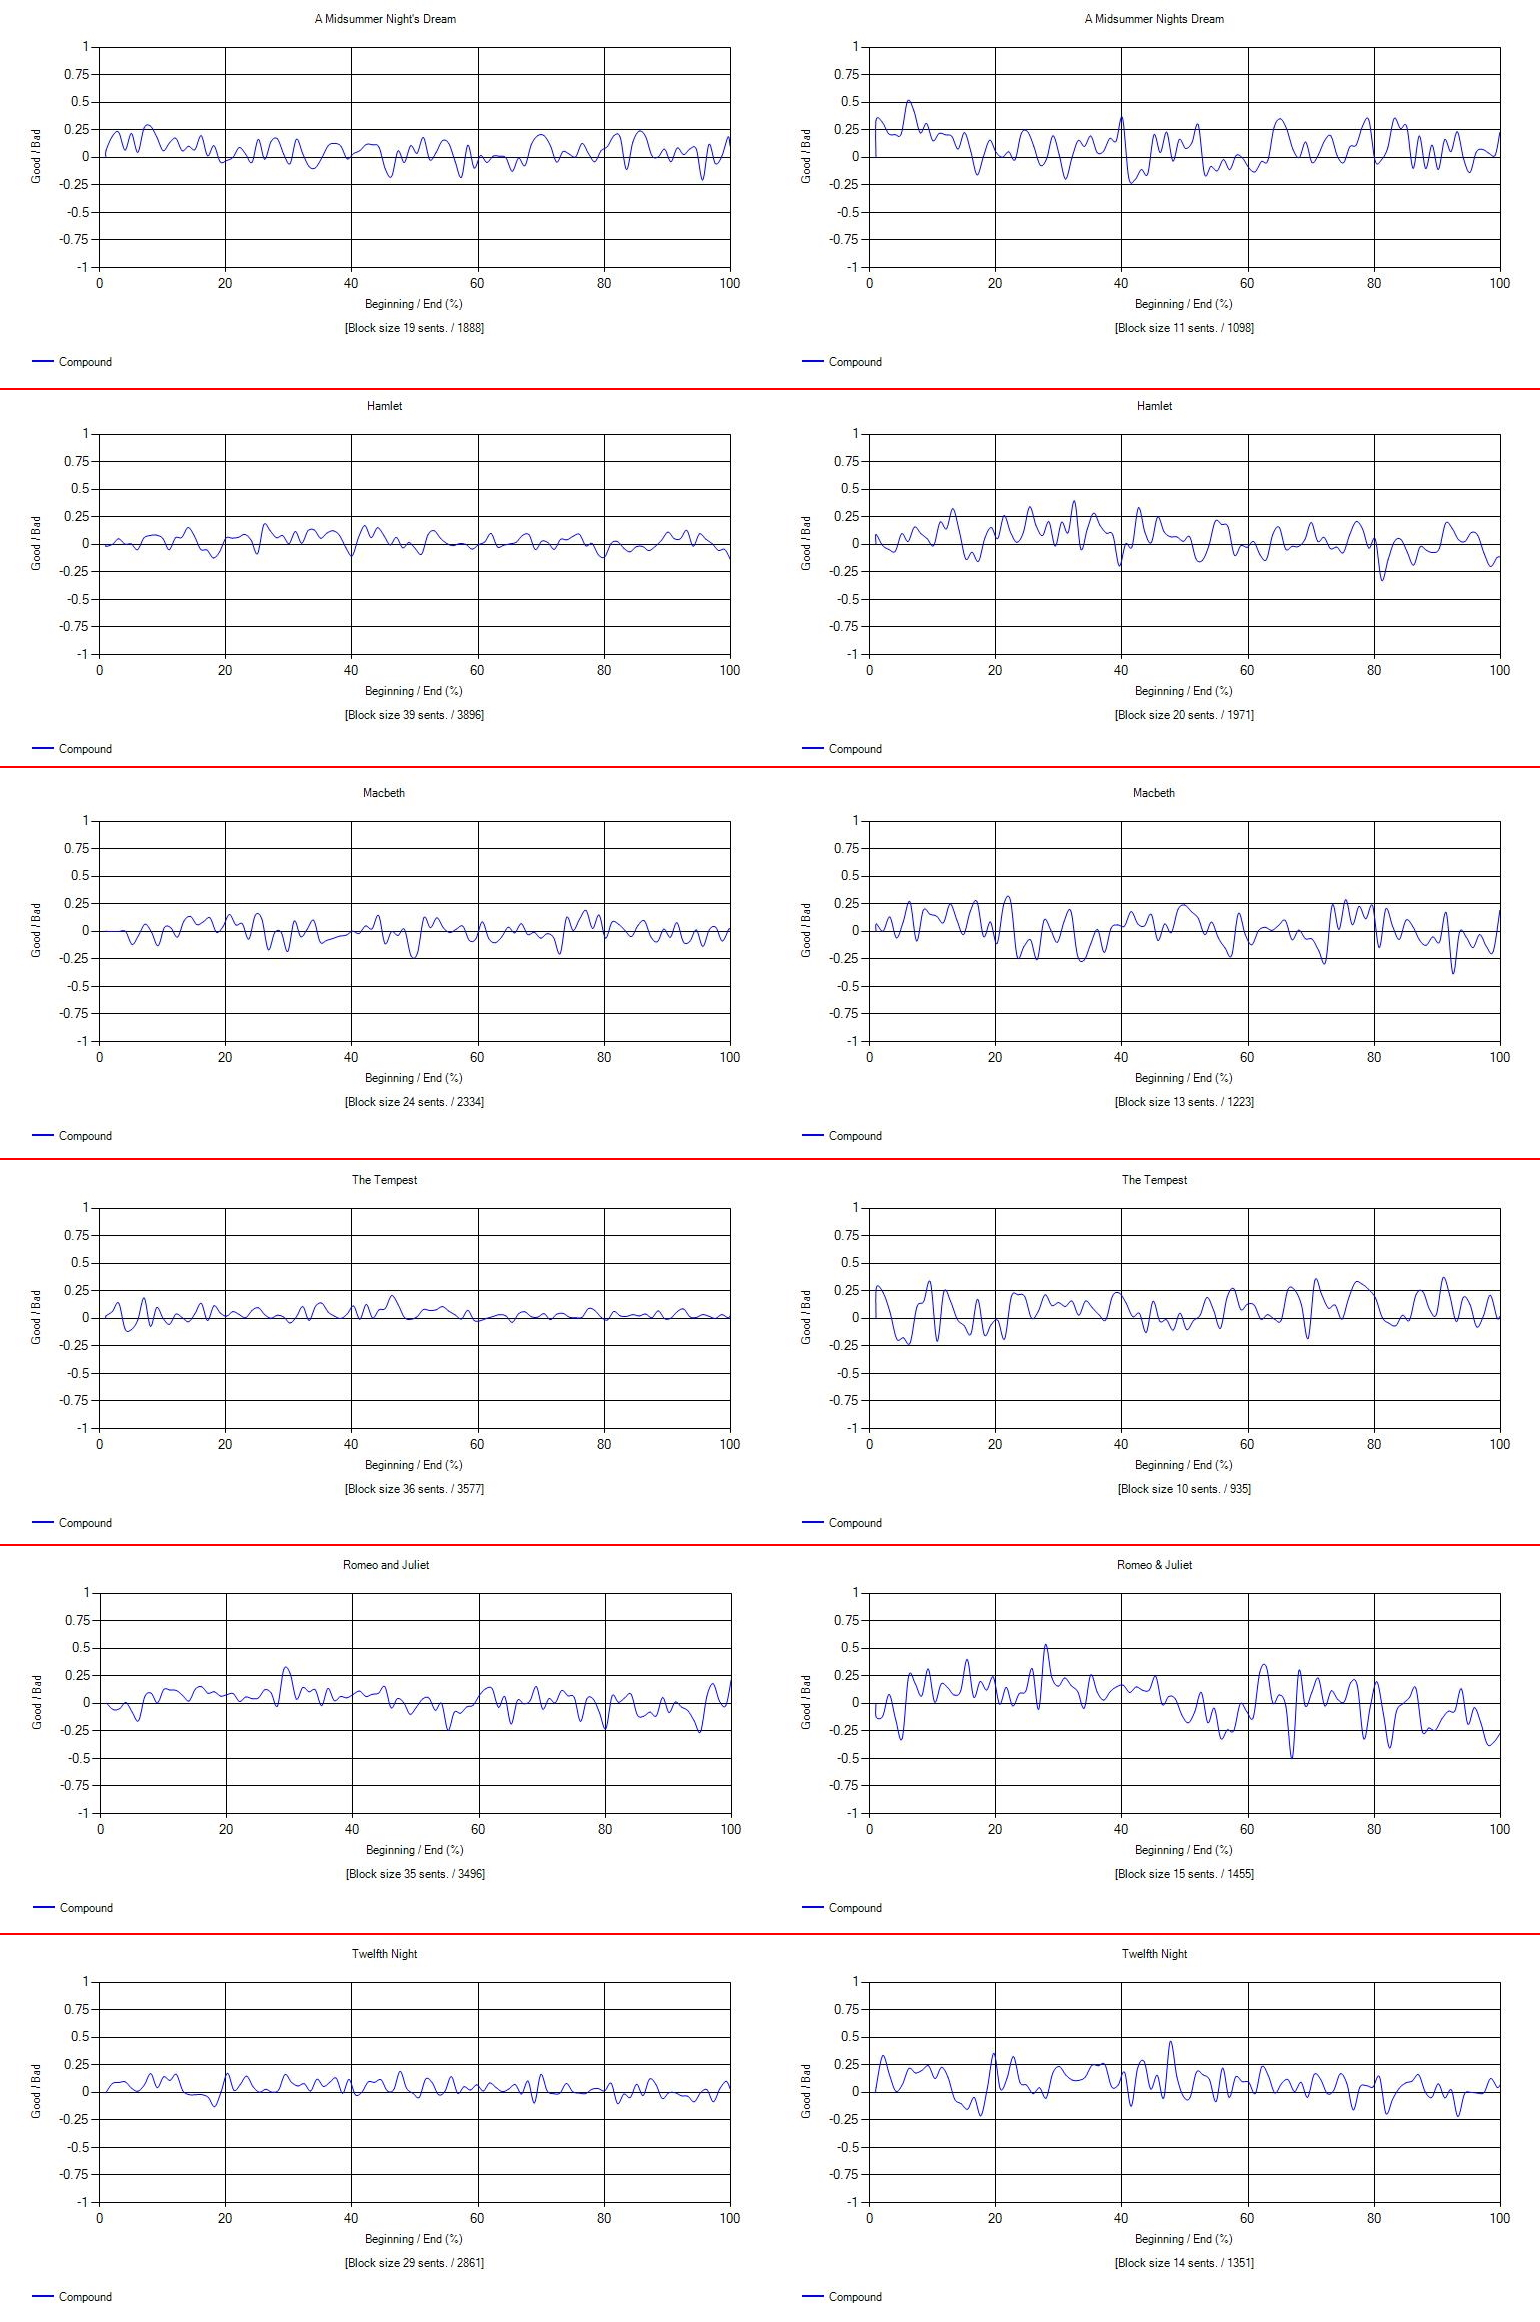
\includegraphics[width=1\textwidth]{Figures/EMvsM/EMvsMAll}
            \centering
            \caption{Original (early modern English) text graphed on the left, along side hand-modernised text on the right for the six varded texts.}
            \label{fig:emvsm}
        \end{figure}
    % \subsection{Shakespeare: Comedies Vs. Tragedies}
    % \label{subsec:comVsTrag}
    %     As mentioned in section \ref{subsec:reader}, Shakespeare plays have been a key source of analysis text. These have generally yielded somewhat restricted graphs. The motivation for these tests came from the thought to force the ability to tell apart different plays by their genre. Namely to comedies \textit{should} show generally more positive curves and similarly, tragedies \textit{should} show more negative curves accordingly. To attempt to display this, three comedies (\textit{Twelfth Night, The Tempest, A Midsummer Night's Dream}) and three tragedies (\textit{Macbeth, Hamlet, Romeo and Juliet}) were processed to give their respective graphs. There is some debate on the specific genre of \textit{The Tempest}, it now often being referred to as a ``late romance'', a subsection of Shakespeare's comedies leaning more toward a ``tragicomedy'' in genre. Nonetheless it ought to still produce a difference in curve to that of the three tragedies.
\newpage
\section{Conclusion}
    This study has covered a range of topics around natural language processing and sentiment analysis in the context of fiction, both in the form of novels and play scripts. Tests were carried out to shed light on the ideal granularity of sentiment analysis in this domain and an effective range was found to be between 0.2\% and 2\% of the length of the corpus being processed.
    
    Efforts were made to identify curves in literature in accordance with Kurt Vonnegut's predictions as laid out in his Master's thesis. While a clear \textit{and} expected curve was found in \textit{Cinderella}, the majority of the graphs produced did not show a \textit{clear} curve, though the door remains open for further research and investigation. Likewise, obvious curves could not be identified within chapters of the same texts. That being said chapter splitting was not achievable for a majority of texts and so there is still much to be explored.
    
    A small analysis was conducted to attempt to assess how effective VADER has been on a per sentence basis and sadly, results came back somewhat negative, with notably less than 50\% of hand-scored sentences having discrepancies of greater than 0.25. These results were less than impressive, yet by the time this was discovered, it was too late to swap out VADER for another tool. That being said, future extension to Sentiplot could implement this.
    
    To further check VADER's results and to marry this to attempts to identify curves, a survey was carried out with participants identified primarily as students with specialist knowledge around English Literature and Language and Shakespeare through theatre. Concerned directly with Shakespeare plays, the survey comprised two sections: firstly to show what participants thought the curves of a given text would be and secondly to compare this with the curves produced by Sentiplot. Quite rightly upon looking at the presented graphs, most participants commented on how Sentiplot's graphs seemed all to look very similar to each other or otherwise bore little to no resemblance of what they thought should be shown. It was suggested that the poor variation between the graphs might be attributed to the fact that the text used to produce the graphs was a play script, which by nature contains very little (sentiment carrying) description by comparison to a novel or similar.

    One of the most interesting and unique experiments was the final experiment which compared the results of Sentiplot when processing Shakespeare plays in their original early modern English spelling with the results of those same plays converted to modern English by VARD. The resultant graphs showed that the VARDed texts produced much more varied results, in all case exaggerating the previously narrow-range graphs and revealing a number of additional features in a few texts.\footnote{``This may be one of the first, if not \textit{the} first comparison of sentiment analysis tools [on corpora] with and without VARD/spelling normalisation.'' - Paul Rayson, in personal communication}
    \subsection{Review of Aims}
        The following list repeats the aims presented at the start of this report, with each aim followed by an overview of relevant results obtained.
        \begin{itemize}
            \item \textcolor{gray}{\textit{Design and develop an application to process a range of corpora to produce a graphing of the emotional arc during its literary course (as produced using SA)}}
            
            The Sentiplot tool functionally fulfilled this aim acceptably. It is able to parse text in a small number of formats, pre-process it and hand it to VADER such that the results may be plotted on a set of axes. And it successfully facilitated the experimentation present in this report.

            \item \textcolor{gray}{\textit{Analyse a range of corpora for compliance with Kurt Vonnegut’s theories and story shapes}}
            
            A small variety of corpora was processed for compliance and similarity. There was certainly scope for more texts to be analysed, however the lack of positive results and the inconsistencies of Project Gutenberg's format (see figures \ref{subsec:curves} \& \ref{subsec:gutenbergFormat}) prompted a halt to in-depth experimentation.
            \item \textcolor{gray}{\textit{Otherwise attempt to identify potential trends in the texts processed, such as obvious geometric differences between literature generally considered happy/sad}}
            
            Of the texts produced, \textit{Cinderella} was the sole text to produce a visibly similar graph to to that predicted by Kurt Vonnegut. This aim was attempted and was found unsuccessful.
            \item \textcolor{gray}{\textit{Present graphs of texts to readers who are familiar with the text to assess if their perceptions of the text align with the SA graphs}}
            
            A survey of readers was carried out, obtaining 22 sets of results that was used for side-by-side analysis with VADER's graphs but also for self-analysis and comments around the Sentiplot tool.
            \item \textcolor{gray}{\textit{Assess VADER's ability to process text outside its design remit (e.g. early-modern English)}}
            
            This aim was fulfilled directly via the processing of the varded Shakespeare texts. It was shown that VADER does indeed perform better on modern English.
        \end{itemize}
    \subsection{Reflections}
        \subsubsection{Deviation From Original Plans}
            The original main premise of this study had been to identify if and thus to what extent, various pieces of literature could be shown to have emotional curves. These were then to be compared a number of shapes as defined by Kurt Vonnegut. After early results came back, it was shown that this might prove to be more problematic than at first thought. Consequently, the focus of the project was widened to cover a broader remit, leading to the experiments presented in section \ref{sec:experiments}. As the project went on, each stage of progress tended to lead to the next stage quite natural, one experiment requiring first some other information. In this way, the project was self-exploring to a small degree.

            While it is unfortunate that curves could not be easily deduced from stories here, the novel origins remained present and still allowed a range of new research to be carried out in the field of NLP for fiction.
        \subsubsection{Revisions to System}
            Given the results obtained from VADER, it is likely that a different sentiment analysis engine may produce better results. This stems from a number of reasons, not least that VADER was originally designed for short input texts (the length of a Tweet) but also that it was trained on modern English text, not the early-modern English found in Shakespeare's plays. More advanced and versatile NLP and sentiment analysis tools may be better able to yield results on the topic

            As detailed in section \ref{subsec:gutenbergFormat}, the format of corpora taken from Project Gutenberg varied in such a way that the Sentiplot tool was unable to effectively and reliable strip away unwanted text bloat before submitting it to be processed. This visually affected results at key points (the beginning and end of some graphs), causing confusion and misunderstanding amongst some of the participants in section \ref{subsec:reader}. An alternate, more consistent source of corpora must be found or the Sentiplot tool must be developed further to account for this inconsistency. This may mean that chapter analysis may have to be scrapped or very much non-trivial algorithms must be implemented to correctly divide texts at appropriate chapter boundaries.
        \subsubsection{Project Process}
            I conducted this project over the course of 20 weeks (plus four weeks during the Christmas holidays) from Early October through till mid March. The original Gantt chart (See Appendix) projected an implementation completion by the end of the first 10 weeks. While the initial design was completed in a good time, due to a range of factors outside the project remit, the development phase overran by 3 weeks, consequently pushing back the development of experiment features and further work. Fortunately, enough buffer was planned in the final-write up stage that this was easily absorbed. In future, I need to ensure my time is well balanced between academic commitments - even if a deadline is further away, a project such as this cannot be left idle so often.

            I did not dedicate enough time to selecting corpora, overestimating the standardisation of Project Gutenberg which later led to some minor issues during feature development. As mentioned in section \ref{subsec:gutenbergFormat}, the formatting of the texts collected varied enough to cause noticeable discrepancies in the results due to the parser for the HTML files not being written to account for the format they were provided in. Though it had a less impactful effect on most of the results, this was problematic under the topic of chapter identification where this often produced chapters without meaningful text or failed entirely. More time needed to be dedicated to this in order for this function to work fully.
    \subsection{Negative Impacting Circumstances}
        During the final stages of the project, I was affected by two major events that took non-trivial lengths of time away from progressing my work.

        First, the death and subsequent funeral of an immediate family member took place in week 18, for which I needed to return home. I was unable to work from the evening of Thursday 5th till midday Sunday 8th due to lack of access to my computer and resources and travel.

        Secondly, week 20 saw the entire country's education system begin to be directly pressured by the outbreak the Coronavirus COVID-19. Thankfully, my supervisor Paul Rayson and other involved parties were able to provide seamless assistance despite the fact I needed again to return home from Lancaster early. This did however still result in a loss of time between midday Tuesday 17th and the afternoon of Wednesday 18th, due to travel, in the run up to the deadline.
    \subsection{Future Research}
        There is scope for further research here, particularly around the comparison of NLP tool performance on different variations of English as in section \ref{subsec:EMvME}. This showed promise in the very obvious and clear improved performance when processing the varded text over the original. It could be explored if other tools perform better on this form of English by default, or failing that, if user-trainable tools could be taught how to process early-modern English to an equal standard.

        Sentiment analysis as a method overall may be tested in its own right for practicality to this. Seeing how the Hedonometer Project applies SA, a bag-of-words type approach, it appears that although more basic, SA is quite attuned to this seeing as how it does not take much of any context into account. The emotional methods as used in LIWC and deeper machine learning techniques may have the potential to take this subject matter much further than sentiment analysis alone.
    \subsection{Closing Statement}
        The initial goal of this study may have changed significantly early on, however this report has still made fresh footprints in the region of NLP in the domain of fiction and for alternative forms English, particularly with regards to comparison of texts with and without normalised spelling. Although inferable from the underlying methods, this report goes some way to proving that normalised spelling allows NLP tools like sentiment analysis to perform better.

        I have personally learnt a lot throughout the project's course, particularly in the fields of natural language processing and sentiment analysis. I have acquired new skills around project and time management and academic writing. Despite the great gains in knowledge for myself, I believe I have also produced a report that may provide a launchpad for other more in-depth studies in the same field.
        
        Overall, I feel this study has been a success and that I have grown both personally and academically in light of its completion.s
\label{sec:conclusion}
\newpage
\bibliography{ref}
\newpage
\section*{Appendix}
    \subsection*{Appendix 1: Project Proposal}
        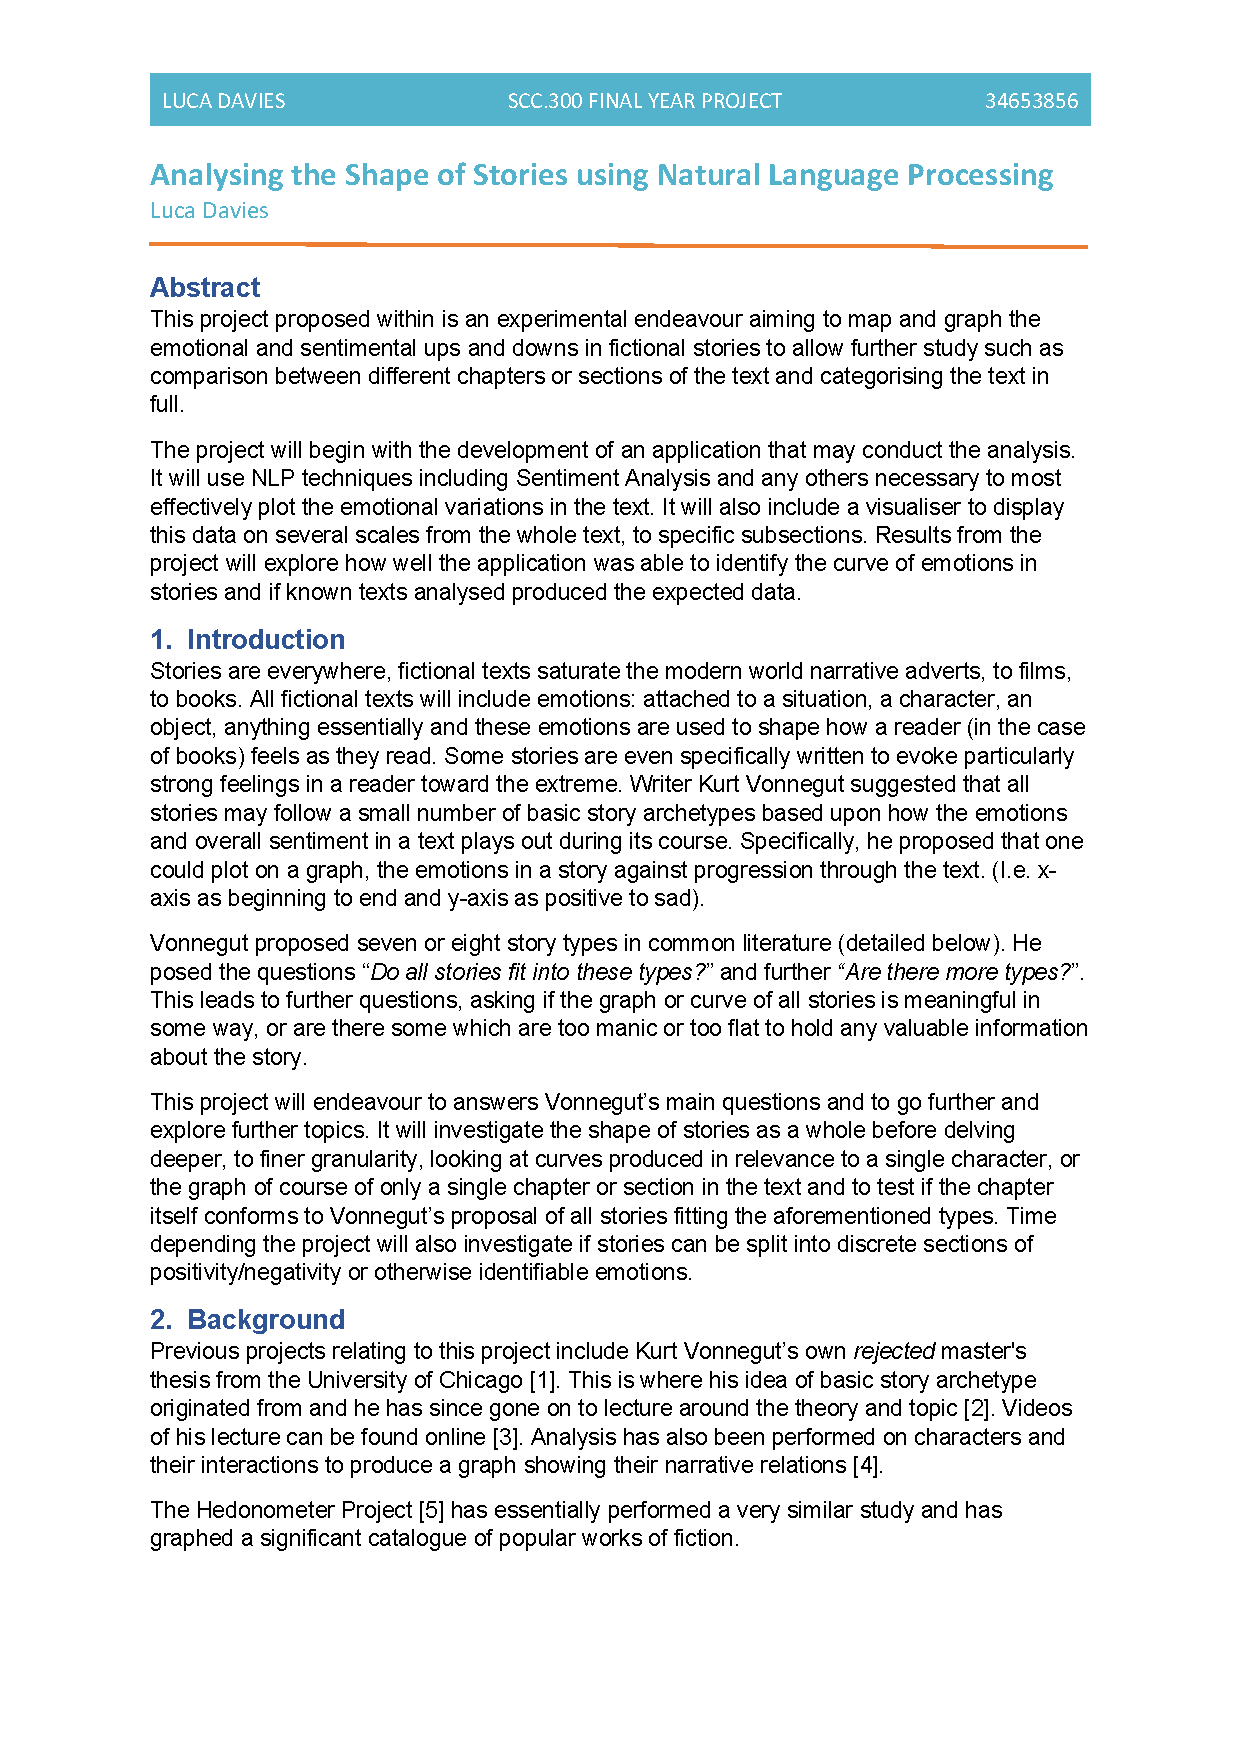
\includepdf[pages=-]{Proposal/SCC.300 Project Proposal}
    \subsection*{Appendix 2: Participants Study Questionnaire}
        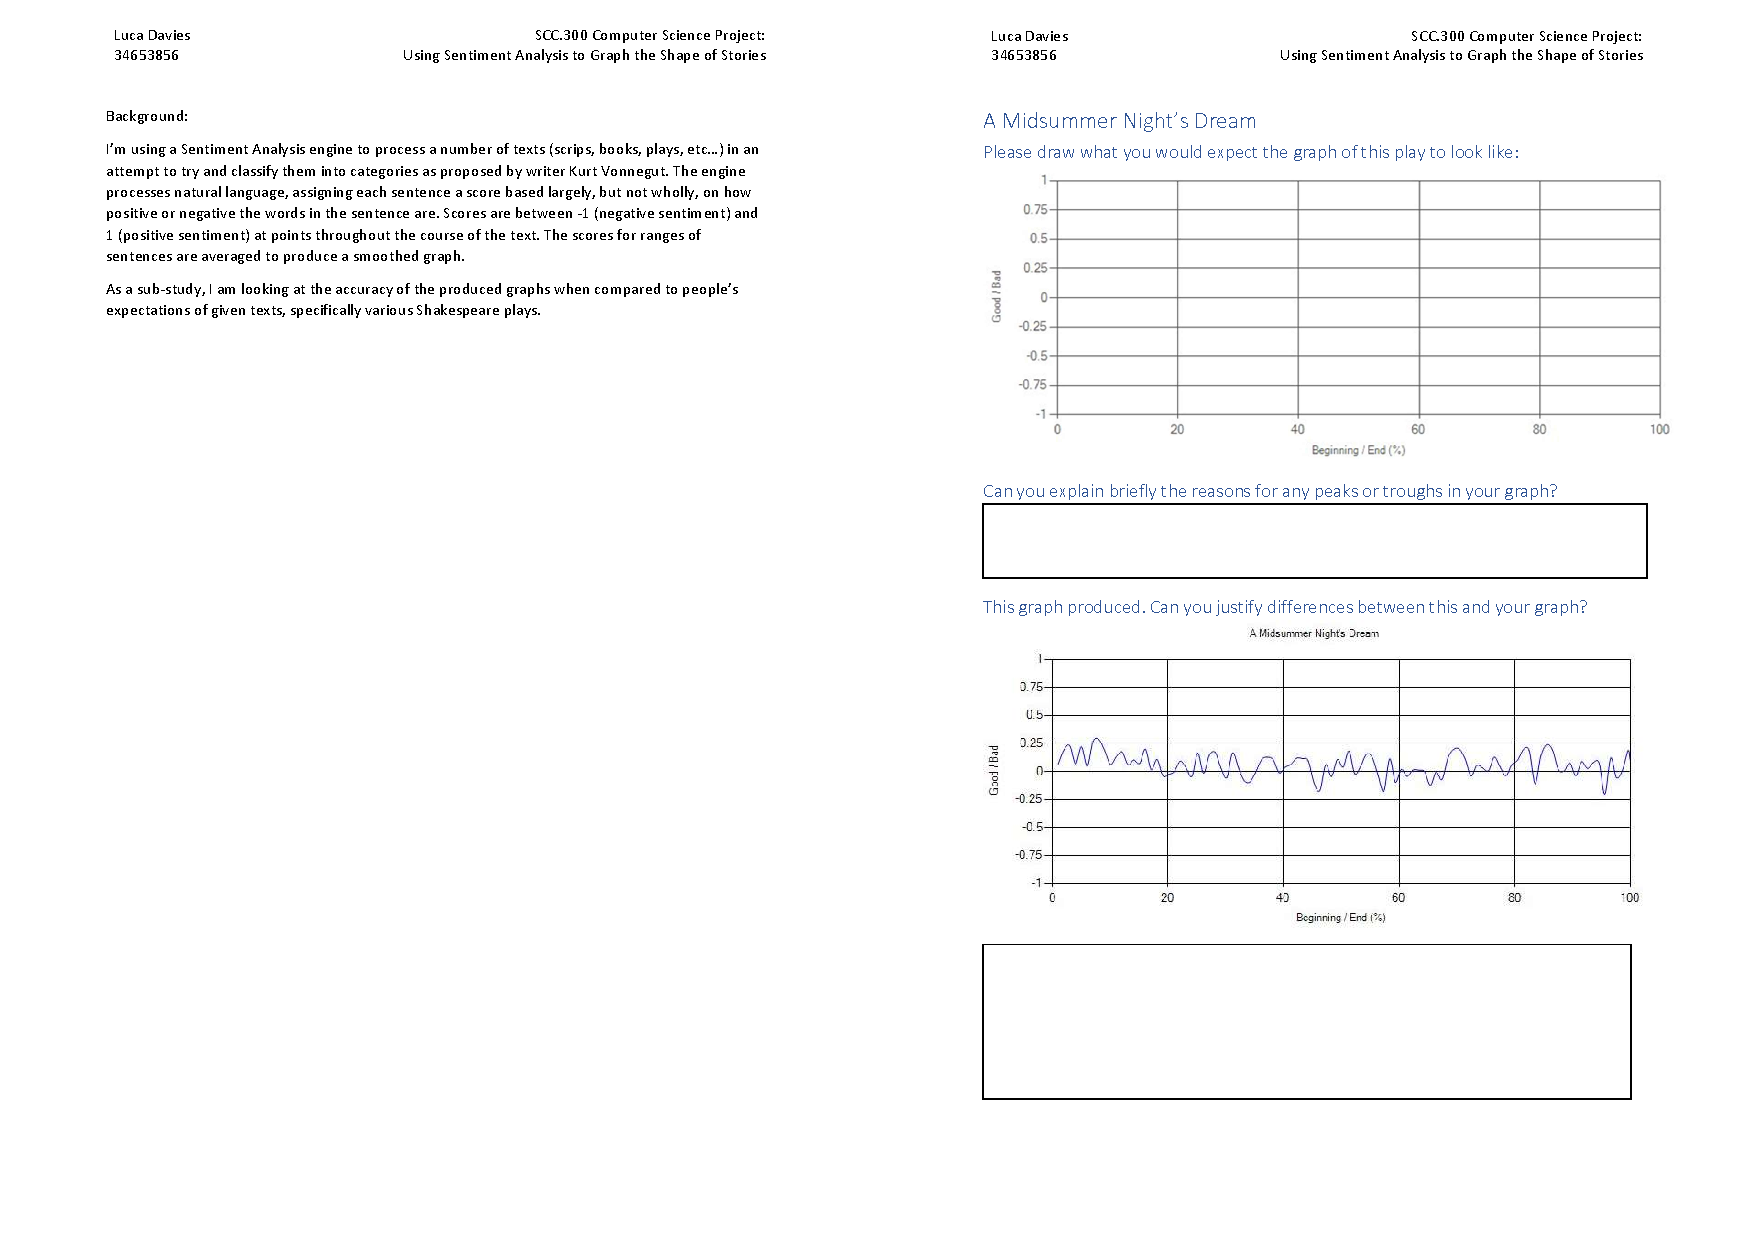
\includegraphics[width=1.5\textwidth, angle=90, origin=c]{Figures/Survey/Questionnaire}
\end{document}
